\section{Power Variability}
\label{sec:variability}

As fabrication technologies improve and feature sizes decrease, hardware variation plays an increasingly important role in determining the power consumption and therefore lifetime of computer systems. This variability can be attributed to: manufacturing (due to scaling of physical feature dimensions faster than optical wavelengths and equipment tolerances~\cite{Bernstein:2006,Cao:2002}); environment (e.g. voltage and temperature); aging (e.g. due to negative bias temperature instability \cite{Zheng:2009}); and vendors (multi-sourcing of parts with identical specifications from different manufacturers). 


Power consumption in an embedded processor can be classified as either active power or sleep (idle) power. Active power includes switching and short-circuit power and can be modeled as in~\cite{RabaeyCN96} and \cite{Veendrick84}:


\begin{equation}
P_{a} ={C} V_{dd}^2f + {\eta(V_{dd}-V_{thn}-V_{thp})^3f}
\label{equ:switching_power}
\end{equation}



\noindent where $C$ is the switching capacitance, $V_{dd}$ is the operating voltage, $f$ is the clock frequency, $\eta$ is a technology- and design-dependent parameter, $V_{thn}$ is the threshold voltage for NMOS,
and $V_{thp}$ is the threshold voltage for PMOS.
% and equals $|V_{thp0}+\Delta V_{thp}|$, $V_{thp0}$ is the threshold voltage without degradation.
The threshold voltage $V_{thp}$ is subject to wear-out due to negative bias temperature instability (NBTI) as described in~\cite{ChenWC12,BhardwajWV06,WangYB07}.
%
Sleep power can be modeled as 

\begin{equation}
P_{s} = V_{dd} (I_{sub}+I_{g})
\end{equation}

where $I_{sub}$ is the sub-threshold leakage current and $I_{g}$ is the gate leakage current. Sub-threshold leakage current models can be derived from the device model in~\cite{BSIM}, and simplified to extract its temperature and voltage dependency:

\begin{equation}
I_{sub} = a_{1} T^2 \left(\exp\left(\frac{-a_{2}V_{thp}}{T}\right)+\exp\left(\frac{-a_{2}V_{thn}}{T}\right)\right)\exp\left(\frac{-a_{3}V_{dd}}{T}\right)
\end{equation}
where $T$ is temperature in Kelvin and $\{a_{1}, a_2, a_3\}$ are empirically fitted parameters that capture part-to-part variations. Gate leakage current is defined in ~\cite{KimAB03} as:

\begin{equation}
I_{g} = a_{4} V_{dd}^2 \exp(-a_{5}/V_{dd})
\end{equation}
%
where $a_{4}$ and $a_5$ are empirically fitted parameters.



While the large baseline in active power consumption relative to idle power consumption amortizes  variations to some degree (\cite{Wanner:2012} cites a 10\% variation in active power while \cite{balaji2012} cites between 7\% and 17\% variation), the low baseline in idle power consumption renders it highly susceptible to fabrication-induced variations (\cite{Wanner:2012} reports a 14x range in measured idle powers across 10 instances of ARM Cortex M3 processors in 130nm technology). 

\begin{figure}
\centering
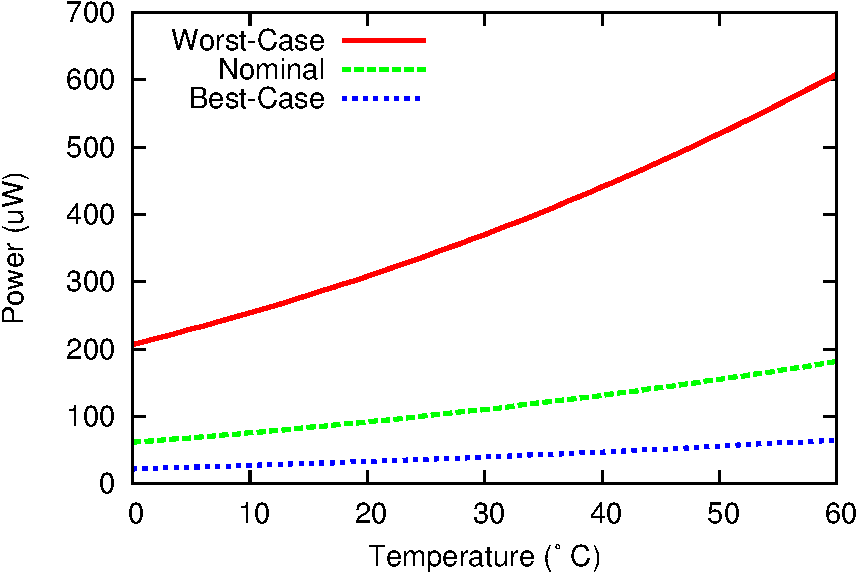
\includegraphics[width=0.48\textwidth]{figures/sleep_power}
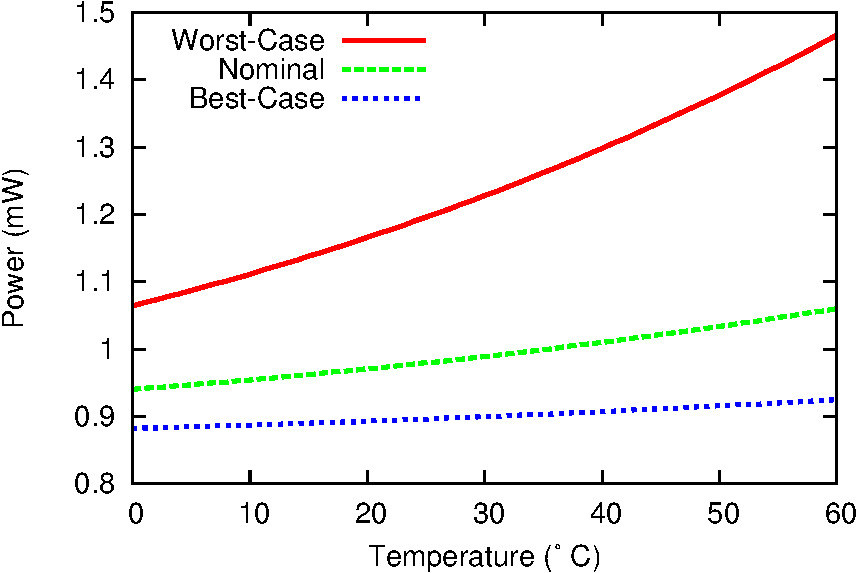
\includegraphics[width=0.48\textwidth]{figures/active_power}

\caption{\label{fig:power}Sleep (left) and Active (right) power for three processor instances in 45nm representing the range of variation for the technology.}
\end{figure}


In this work, we use 45nm process technology and libraries as our baseline for evaluation. Power model parameters are fitted to the SPICE simulation results of an inverter chain using the device model given in the technology libraries.  The final power values are normalized to the measured data obtained from an M3 test chip using the same technology. Figure~\ref{fig:power} shows active and sleep power across temperature for three instances representing the range of power variation for this technology (nominal, worst-case, and best-case).  At room temperature, there is approximately 6x variation in sleep power consumption between the worst- and best-case instances. This magnitude of variation matches measurements with off-the-shelf embedded class processors fabricated in 130nm shown in \cite{Wanner:2012}, and hence represents a conservative estimation of the variation that may be found in processors in newer technologies. 

Power consumption in energy-constrained embedded systems is often dominated by time spent in an idle state.  Consequently, the lifetimes of these systems can be widely variant due to instance-to-instance variation in idle power, resulting in either premature system death or suboptimal system quality and an energy surplus. 

%he result of inaccurate lifetime estimates obtained by improper power models can be one of two things: conservative designs can ensure that lifetime goals are met by adding a guard band to system duty cycle and thus underperforming, or removing these guard bands will result in higher performance while all subsystems (perhaps nodes in a network) are still running, but upon depletion of energy reserves by those processors with higher power consumption the entire system will again suffer.  A processor-specific duty cycle can be assigned so that all lifetimes are met, but without a strategy for distributing resources to individual tasks on a processor there is no guarantee that these variations are handled elegantly and in a way that maximizes application utility. The problem, then, becomes one of maximizing an application's utility while meeting lifetime and energy constraints despite hardware variability. 



